\documentclass[10pt, oneside, letterpaper]{article}
\usepackage[margin=1in]{geometry}
\usepackage[english]{babel}
\usepackage[utf8]{inputenc}
\usepackage{xcolor}
\definecolor{mygreen}{rgb}{0,0.6,0}
\definecolor{mygray}{rgb}{0.5,0.5,0.5}
\definecolor{mymauve}{rgb}{0.58,0,0.82}
\usepackage{listings}
\lstset{
  backgroundcolor=\color{white}, % choose the background color
  basicstyle=\footnotesize\ttfamily, % size of fonts used for the code
  breaklines=true, % automatic line breaking only at whitespace
  frame=single, % add a frame
  captionpos=b, % sets the caption-position to bottom
  commentstyle=\color{mygreen}, % comment style
  escapeinside={\%*}{*)}, % if you want to add LaTeX within your code
  keywordstyle=\color{blue}, % keyword style
  stringstyle=\color{mymauve}, % string literal style
}
\usepackage{enumitem}
\usepackage{blindtext}
\usepackage{datetime2}
\usepackage{fancyhdr}
\usepackage{amsmath}
  \newcommand{\angstrom}{\textup{\AA}} % for units of angstrom
\usepackage{arydshln} % dash line package for matrices
\usepackage{mathtools} % for things like \Aboxed
\usepackage{float}
\usepackage{pgf}
\usepackage{enumitem} % to easily change style of counters in item lists
\usepackage{xurl} % to easily insert URLs in the LaTeX source
\usepackage{braket} % for bra-ket notation
\usepackage{bm} % for bold vector variables
\usepackage{cases} % for piecewise definitions
\usepackage[makeroom]{cancel} % for crossing out terms
\usepackage{graphicx} % for \scalebox
  \newcommand\scalemath[2]{\scalebox{#1}{\mbox{\ensuremath{\displaystyle #2}}}}

\setcounter{MaxMatrixCols}{32} % increase the maximum number of matrix columns

\title{Assignment 2}
\author{Electronic Structures of the Helium atom and Hydrogen Molecule}
\date{Due: 2022/02/11}

\pagestyle{fancy}
\setlength{\headheight}{23pt}
\setlength{\parskip}{1em}
\fancyhf{}
\chead{Assignment 2}
\rhead{Michel Kakulphimp \\ Student \#63542880}
\lhead{ELEC542 \\ UBC MEng}
\cfoot{\thepage}

\begin{document}
\maketitle
\thispagestyle{fancy}

\section{Directions}

The goal in this assignment is to calculate the electronic structure of the helium atom and the hydrogen molecule (two separate systems). The distance between the two hydrogen atoms (the bond length) is 0.74 \angstrom. In this assignment, do not perform geometry optimization, and instead use that fixed bond length in order to calculate the molecular orbitals (both energies and wave functions). Also, note that the problem is in full 3-dimensional space. The goal is to solve the Hartree-Fock equation for these two systems.

Note that you are solving an iterative problem. The Fock operator depends on the orbitals, which you do not have. So, start by making a guess for the orbital shapes, form the Fock operator, solve for the orbitals, and keep iterating until convergence. Use the convergence of the total energy of the system as your convergence criterion.

In this assignment, the calculations must be done directly on a real-space grid, over which the orbitals (wave functions) are defined. So, do not use the Roothaan equations (which we will see soon).

\begin{enumerate}[label=(\alph*)]
  \item (7 points) Directly discretize the Fock operator to put it into matrix form. Describe your approach and show the steps of your derivation all the way to obtaining the matrix equation.
  \item (5 points) Write a computer code to implement what you built in part (a).
  \item (4 points) Plot several molecular orbitals and give their associated energies for the helium atom. Also calculate the total energy of the system (not including the nucleus-nucleus interaction). Discuss your results.
  \item (4 points) Plot several molecular orbitals and give their associated energies for the hydrogen molecule. Also calculate the total energy of the system (not including the nucleus-nucleus interaction). Discuss your results.
\end{enumerate}

\section{Derivation of Solution}

\subsection{Hartree-Fock Matrix Equation Derivation}

Since both subjects for this assignment have an even number of electrons that close shells, we can use the restricted Hartree-Fock equation for closed shell systems to numerically calculate the resulting orbitals. The equation is as follows:

\begin{align*}
  \hat{F}(\vec{r})\psi_n(\vec{r}) &= \epsilon_n\psi_n(\vec{r})
\end{align*}

Where $\hat{F}(\vec{r})$ is the Fock operator which is defined as follows:

\begin{align*}
  \hat{F}(\vec{r}) &= \hat{H}_{core}(\vec{r}) + \sum_{n=1}^{N/2}\left[2J_n(\vec{r}) - K_n(\vec{r})\right]\\
\end{align*}

The Fock operator is composed of the core Hamiltonian operator $\hat{H}(\vec{r})$, the Coulomb operator $\hat{J}(\vec{r})$, and the exchange operator $\hat{K}(\vec{r})$. $P_2$ is a transposition operator which switches the indices of the electron indices, something required by the exchange operator.

\begin{align*}
  \hat{H}_{core}(\vec{r}) &= -\frac{1}{2}\nabla_1^2 - \sum_A\frac{Z_A}{\|\vec{r}_{1 A}\|}\\
  \hat{J}_j(\vec{r}_1)\psi_i(\vec{r}_1) &= \psi_i(\vec{r}_1)\int_{-\infty}^{\infty}\left|\psi_i(\vec{r}_2)\right|^2\frac{1}{\|\vec{r}_{12}\|}d\vec{r}_2 \\
  \hat{K}_j(\vec{r}_1)\psi_i(\vec{r}_1) &= \psi_j(\vec{r}_1)\int_{-\infty}^{\infty}\frac{\psi_j^\ast(\vec{r}_2)\psi_i(\vec{r}_2)}{\|\vec{r}_{12}\|}d\vec{r}_2 \\
\end{align*}
Expanded, the Fock operator takes the following form:

\begin{align*}
  \hat{F}(\vec{r}) &= -\frac{1}{2}\nabla_1^2 - \sum_A\frac{Z_A}{\|\vec{r}_{1 A}\|} + \sum_{n=1}^{N/2}\left[2\int_{-\infty}^{\infty}\left|\psi_n(\vec{r}_2)\right|^2\frac{1}{\|\vec{r}_{12}\|}d\vec{r}_2 - \int_{-\infty}^{\infty}\frac{\psi_n^\ast(\vec{r}_2)P_2\psi_n(\vec{r}_2)}{\|\vec{r}_{12}\|}d\vec{r}_2\right]
\end{align*}

For the Helium atom, the Fock operator takes the following form:

\begin{align*}
  \hat{F}(\vec{r}) &= -\frac{1}{2}\nabla_1^2 - \frac{2}{\|\vec{r}_{1 A}\|} + \int_{-\infty}^{\infty}\left|\psi_1(\vec{r}_2)\right|^2\frac{1}{\|\vec{r}_{12}\|}d\vec{r}_2
\end{align*}

and for the Hydrogen molecule, the Fock operator takes the following form:

\begin{align*}
  \hat{F}(\vec{r}) &= -\frac{1}{2}\nabla_1^2 - \frac{1}{\|\vec{r}_{1 A}\|} - \frac{1}{\|\vec{r}_{1 B}\|} + \int_{-\infty}^{\infty}\left|\psi_1(\vec{r}_2)\right|^2\frac{1}{\|\vec{r}_{12}\|}d\vec{r}_2
\end{align*}

For the ground state, we only consider one orbital to fill, which simplifies the exchange operator's index-switch operator in both Fock operators. This also has the effect of making the Coulomb and exchange integrals identical, greatly simplifying the equation. Note that: $\psi_n^\ast(\vec{r}_2)\psi_n(\vec{r}_2) = \left|\psi_1(\vec{r}_2)\right|^2$. For the Helium atom, our value for $Z_A$ is 2 as there are two protons in the nucleus and for the Hydrogen molecule, we consider both Hydrogen nuclei containing one proton each, so $Z_A = Z_B = 1$. The nuclei are separated by 0.74 \angstrom. Since we are solving this problem using Hartree atomic units, we must convert this value accordingly when considering the coordinates of the hydrogen nuclei. In Hartree atomic units, the atomic unit of length converts the Bohr radius $a_0$ to $1$. Therefore, the distance between the two Hydrogen nuclei is $\frac{0.74 \times 0.1\times10^{-9}}{5.29177210903\times10^{-11}} = 1.39839733222307$ atomic units of length.

In order to discretize these equations, the second order differentiation and the finite integration must be numerically performed, in the three spatial dimensions $x$, $y$, and $z$. For the second order differentiation, it will discretize in the following manner:

\begin{align*}
  \nabla^2f(x, y, z) \approx \frac{f(x + \Delta x,y,z) - 2f(x, y, z) + f(x - \Delta x,y,z)}{\Delta x^2}\\
  + \frac{f(x,y + \Delta y,z) - 2f(x, y, z) + f(x,y - \Delta y,z)}{\Delta y^2}\\
  + \frac{f(x,y,z + \Delta z) - 2f(x, y, z) + f(x,y,z - \Delta z)}{\Delta z^2}
\end{align*}

If we choose the same discretization size, such that $\Delta x = \Delta y = \Delta z = h$, the discretization takes the following simplification:

\begin{align*}
  \nabla^2f(x, y, z) \approx \frac{f(x+h,y,z) + f(x,y+h,z) + f(x,y,z+h) - 6f(x, y, z) + f(x-h,y,z) + f(x,y-h,z) + f(x,y,z-h)}{h^2}\\
\end{align*}

As seen in the previous assignment, by forming a column vector in the following form:

\begin{align*}
  \ket{\psi} = \left[\psi(0,0,0), \hdots ,\psi(N,0,0),\psi(0,1,0),\hdots,\psi(N,1,0),\hdots,\psi(0,N,0),\hdots,\psi(N,N,N)\right]^T
\end{align*}

The indices found in this vector will depend on the limits chosen for the solution in all directions, as well as the number of partitions $N$. With three dimensions and $N$ discretization points, the total number of equations to solve will be $N^3$. The sparse matrix $\bm{S}_{\nabla^2}$ for the Laplacian differential operator on three variables for $N=3$ and $h=1$ is shown below. Three rows have been highlighted to demonstrate how they correspond to an equation in the total solution.

\newpage
\lstinputlisting{sample_sparse_matrix.txt}

The next operator to be considered for discretization is the integration that is performed on the Coulomb and exchange terms. For this integration, we can extend the one dimensional numerical integration intro three dimensions. First we consider the expanded form of the spatial integral:

\begin{align*}
  \int_{-\infty}^{\infty} f(\vec{r})d\vec{r} = \int_{-\infty}^{\infty}\int_{-\infty}^{\infty}\int_{-\infty}^{\infty}f(x,y,z)\,dx\,dy\,dz
\end{align*}

We then split the three spatial dimensions into $N$ partitions in all cardinal directions to quantize the problem into discretized volumes of the solution, $\Delta x$, $\Delta y$, and $\Delta z$ as we did in the differential discretization. Once again, if we choose the same discretization size, such that $\Delta x = \Delta y = \Delta z = h$, we evenly divide the solution space into partitions. By evaluating the function at each coordinate, multiplying the result by our discretization size $h$, and summing over the solution space, we obtain a Riemann sum, which is a trivial implementation of numerical integration. The sums approximate the integral as follows:

\begin{align*}
  \int_{-\infty}^{\infty}\int_{-\infty}^{\infty}\int_{-\infty}^{\infty}f(x,y,z)\,dx\,dy\,dz &\approx \sum_{k_z=0}^N\sum_{k_y=0}^N\sum_{k_x=0}^N \left[w^{[k_x, k_y, k_z]}f(k_x, k_y, k_z)\right] \\
  w_{k_x} = w_{k_y} = w_{k_z} &= \{0, h, h, ..., h\}
\end{align*}

One limitation of this approximated integration is that the infinite limit definite integral required by the original equation is now confined within the limits we choose for the problem and the $N$ partitions we make out of the space in all directions. Choosing the limits and $N$ must be done carefully as the matrices generated for the solution will easily balloon into very difficult diagonalization problems.

Both the Helium atom and the Hydrogen molecule share the following integral term:

\begin{align*}
  \int_{-\infty}^{\infty}\left|\psi_1(\vec{r}_2)\right|^2\frac{1}{\|\vec{r}_{12}\|}d\vec{r}_2
\end{align*}

For every iteration of the Hartree-Fock algorithm, a solution set will be generated for $\psi_1(\vec{r}_1)$ when the Fock matrix $\bf{F}$ is diagonalized. This solution is then re-used in the upcoming iteration as the solution for $\psi_1(\vec{r}_2)$ for use in the integrals. For the first iteration, a version of $\psi_1(\vec{r}_2)$ will be use where every entry is 0. If that fails to converge, then a noisy solution will be attempted. Another thing to take into account is the fact that there will be multiple solutions in the eigenvectors. For every energy to be plotted, that energy's resulting wavefunction will need to be used in each iteration step. Using the sums above, $\psi_1(x_2, y_2, z_2)$ will be evaluated and a value will be obtained. Depending on which energy is being calculated, that energy's eigenvector will be chosen to calculate the integral. This integral also possesses a distance calculation between the current and other electron. This calculation relies on the position of the current step as seen below:

\begin{align*}
  \frac{1}{\|\vec{r}_{12}\|} = \frac{1}{\sqrt{(x_2-x_1)^2 + (y_2-y_1)^2 + (z_2-z_1)^2}}
\end{align*}

This integral will be evaluated for every partition in the problem; therefore, the values for $x_1$, $y_1$, and $z_1$ will correspond to those found in the column vector $\ket{\psi}$ as defined above. This integration operator can be summarized as follows:

\begin{align*}
  I(x_1, y_1, z_1) = \int_{-\infty}^{\infty}\left|\psi_1(\vec{r}_2)\right|^2\frac{1}{\|\vec{r}_{12}\|}d\vec{r}_2
\end{align*}

This equation will form a diagonal in a matrix $J$ of size $N \times N \times N$ as follows:

\begin{align*}
\bm{J} =
\begin{bmatrix}
 I(x_1, y_1, z_1) & 0 & \hdots & 0\\
 0 &  I(x_1, y_1, z_1) & \hdots & 0\\
 \vdots & \vdots & \ddots & 0\\
 0 & 0 & 0 &  I(x_1, y_1, z_1)\\
\end{bmatrix}
\end{align*}

The final term of the Fock equation that needs to be considered is the nuclear attraction operator. For the Helium atom case, we have a single term, and for the Hydrogen molecule we have two terms. For the Helium atom, the expanded nuclear attraction term is as follows:

\begin{align*}
  A_{He}(x_1, y_1, z_1) = -\sum_A\frac{Z_A}{\|\vec{r}_{1 A}\|} = -\frac{2}{\sqrt{(x_1^2 + y_1^2 + z_1^2)}}
\end{align*}

With the Helium nucleus placed at the origin of the problem, the distance between the electron and the nucleus becomes the distance of the electron from the origin. Also, the atomic number for Helium is 2, which puts that number in the denominator.

The Hydrogen molecule on the other hand takes a slightly different form. A hydrogen molecule has two nuclei in its system and they are separated by $1.39839733222307$ atomic units of length as calculated above. For this problem, the Hydrogen nuclei will be placed $\frac{1.39839733222307}{2}$ in the positive and negative $x$ directions from the origin. With an atomic number of 1 for the Hydrogen element, the nuclear attraction terms will take the following form:

\begin{align*}
  A_{H_2}(x_1, y_1, z_1) = -\sum_A\frac{Z_A}{\|\vec{r}_{1 A}\|} = -\frac{1}{\sqrt{(\frac{-1.39839733222307}{2}-x_1)^2 + y_1^2 + z_1^2}} -\frac{1}{\sqrt{(\frac{1.39839733222307}{2}-x_1)^2 + y_1^2 + z_1^2}}
\end{align*}

The nuclear attraction operator will form a diagonal in a matrix $A$ of size $N \times N \times N$ as follows:

\begin{align*}
\bm{A} =
\begin{bmatrix}
 A(x_1, y_1, z_1) & 0 & \hdots & 0\\
 0 &  A(x_1, y_1, z_1) & \hdots & 0\\
 \vdots & \vdots & \ddots & 0\\
 0 & 0 & 0 &  A(x_1, y_1, z_1)\\
\end{bmatrix}
\end{align*}

Now we have all of the components necessary to implement a solution. To summarize, for the Helium atom, the following matrix system will be solved:

\begin{align*}
  \bm{F}_{He}\ket{\psi} = \bm{\epsilon}\ket{\psi} \\
  \bm{F}_{He} = -\frac{1}{2h^2}\bm{S}_{\nabla^2} + \bm{A}_{He} + \bm{J}
\end{align*}

and for the Hydrogen molecule, the following matrix system will be solved:

\begin{align*}
  \bm{F}_{H_2}\ket{\psi} = \bm{\epsilon}\ket{\psi} \\
  \bm{F}_{H_2} = -\frac{1}{2h^2}\bm{S}_{\nabla^2} + \bm{A}_{H_2} + \bm{J}
\end{align*}

\newpage
\subsection{Hartree-Fock Energy Calculation Derivation}

The orbital energies do not sum the Hartree-Fock energy. Koopman's theorem states that in restricted Hartree-Fock, the energies associated with occupied orbitals approximate the ionization energy of that orbital, and the energies associated with unoccupied orbitals approximate the energy required to place an electron into that orbital. The total energy of the system must be calculated using the following equation which accounts for the double contribution of electrons in the double electron integrals (hence the $\frac{1}{2}$):

\begin{align*}
  E_o &= \sum_i^N\bra{i}\hat{h}\ket{i} + \frac{1}{2}\sum_{i>j}^N\left[ij\|ij\right]
\end{align*}

This implies that for the total energy, we can take the expectation value of the resulting Fock operators for both the Helium atom and the Hydrogen molecule, while making sure to halve the contribution of the Coulomb and exchange terms and also using the calculated ground state orbital which both electrons occupy. Also, since both electrons occupy the same spin orbital, terms will end up combining (e.g. $\bra{1}\hat{h}\ket{1} + \bra{1}\hat{h}\ket{1} = 2\bra{1}\hat{h}\ket{1}$)

\begin{align*}
  E_{o(He)} &= E_{o(H_2)} = \sum_i^2\bra{i}\hat{h}\ket{i} + \frac{1}{2}\sum_{i>j}^N\left[ij\middle|ij\right] \\
  &= \bra{1}\hat{h}\ket{1} + \bra{2}\hat{h}\ket{2} + \frac{1}{2}\left(\left[11\middle|22\right] + \left[12\middle|12\right]\right) \\
  &= 2\bra{1}\hat{h}\ket{1} + \frac{1}{2}\left[11\middle|22\right] + \frac{1}{2}\left[12\middle|12\right]
\end{align*}

The total energy for the Helium molecule and Hydrogen atom in their ground states should then be equal to:

\begin{align*}
  E_{o(H_2)} &= 2\int_{-\infty}^{\infty}\psi_1^\ast(\vec{r}_1) \left[ -\frac{1}{2}\nabla_1^2 - \frac{2}{\|\vec{r}_{1 A}\|} \right] \psi_1(\vec{r}_1) d\vec{r}_1 + 
   \frac{1}{2}\int_{-\infty}^{\infty}\int_{-\infty}^{\infty} \psi_1^\ast(\vec{r}_1) \psi_1(\vec{r}_1) \frac{1}{\|\vec{r}_{12}\|} \psi_2^\ast(\vec{r}_2)\psi_2(\vec{r}_2) d\vec{r}_2d\vec{r}_1 \\
   &\qquad + \frac{1}{2}\int_{-\infty}^{\infty}\int_{-\infty}^{\infty} \psi_1^\ast(\vec{r}_1) \psi_2(\vec{r}_1) \frac{1}{\|\vec{r}_{12}\|} \psi_2^\ast(\vec{r}_2)\psi_1(\vec{r}_2) d\vec{r}_2d\vec{r}_1  \\
\end{align*}

\begin{align*}
  E_{o(H_2)} &= 2\int_{-\infty}^{\infty}\psi_1^\ast(\vec{r}_1) \left[ -\frac{1}{2}\nabla_1^2 - \frac{1}{\|\vec{r}_{1 A}\|} - \frac{1}{\|\vec{r}_{1 B}\|} \right] \psi_1(\vec{r}_1) d\vec{r}_1 +
   \frac{1}{2}\int_{-\infty}^{\infty}\int_{-\infty}^{\infty} \psi_1^\ast(\vec{r}_1) \psi_1(\vec{r}_1) \frac{1}{\|\vec{r}_{12}\|} \psi_2^\ast(\vec{r}_2)\psi_2(\vec{r}_2) d\vec{r}_2d\vec{r}_1 \\
   &\qquad + \frac{1}{2}\int_{-\infty}^{\infty}\int_{-\infty}^{\infty} \psi_1^\ast(\vec{r}_1) \psi_2(\vec{r}_1) \frac{1}{\|\vec{r}_{12}\|} \psi_2^\ast(\vec{r}_2)\psi_1(\vec{r}_2) d\vec{r}_2d\vec{r}_1  \\
\end{align*}


% The total energy of the system is defined as follows:

% \begin{align*}
%   E_o &= \sum_i^N\bra{i}\hat{h}\ket{i} + \frac{1}{2}\sum_i^N\sum_j^N\bra{ij}\ket{ij}
% \end{align*}

% Since both electrons of the Helium atom and the Hydrogen molecule both fill a single orbital, the total energy can be expanded as follows for both:

% \begin{align*}
%   E_o &= \bra{1}\hat{h}\ket{1} + \bra{2}\hat{h}\ket{2} + \frac{1}{2}\bra{12}\ket{12}
% \end{align*}

%TODO energy level calculations

\newpage
\section{Program Implementation}

The program for this assignment was written in Python and the source can be viewed in Section \ref{code-listing-python}. It relies heavily on the SciPy package to perform the matrix algebra required to obtain the results. The program constructs the sparse matrices outlined in the previous section, obtains solutions based on convergence criteria, and outputs the plots and data for further analysis.

The program features command line arguments for the user to set various runtime variables and features the ability to load and save the data in a specially formatted file. These files will also contain the configuration values for the simulation run as well as metrics to gauge how quickly each solution was able to converge to a final solution. The user can specify the number of partitions $N$ to use for the problem, resulting in an $N \times N \times N$ sized sparse matrix to calculate eigenvectors and eigenvalues from. Increasing the partition size has a severe impact on performance, so the user must be careful to pick a reasonable size.

In order to optimize the calculations, sparse matrices provided by the SciPy package are used to reduce the memory footprint as well as enable more effective linear algebra operations. All of the sparse matrices are combined together into the Hermitian representing the Fock matrix, and the SciPy \texttt{scipy.sparse.linalg.eigsh} function is used to calculate the associated eigenvalues and eigenvectors. This eigenvalue solver does not fully utilize the capabilities of the computer, using very little CPU time.

Only the lowest six eigenvalues and eigenvectors are calculated for from the Fock matrix. These six eigenvalues are used for the convergence criteria. Their absolute value is summed up, and their percent change is compared from iteration to iteration. If the percent change between two iterations is less than what was specified, the simulation finishes.

The matplotlib Python package is used to generate 4D plots of the resulting orbitals. A 3D scatter plot is used with a heatmap and a mask. The mask allows the plot to selectively ignore points which fall out of a certain range, which allows the plots to effectively illustrate the calculated orbitals. The orbitals are plotted from their lowest energy to the highest energy. Since the resulting waveform will have both negative and positive values, the eigenvector is squared so that the resulting waveform only has positive values. This corresponds to the probability density of the waveform.

A Windows batch file was created to more easily construct simulation runs for execution and data retrieval. The batch file executes concurrent scripts which run in the background.

\newpage
\section{Results}

\begin{figure}[H]
  \begin{center}
    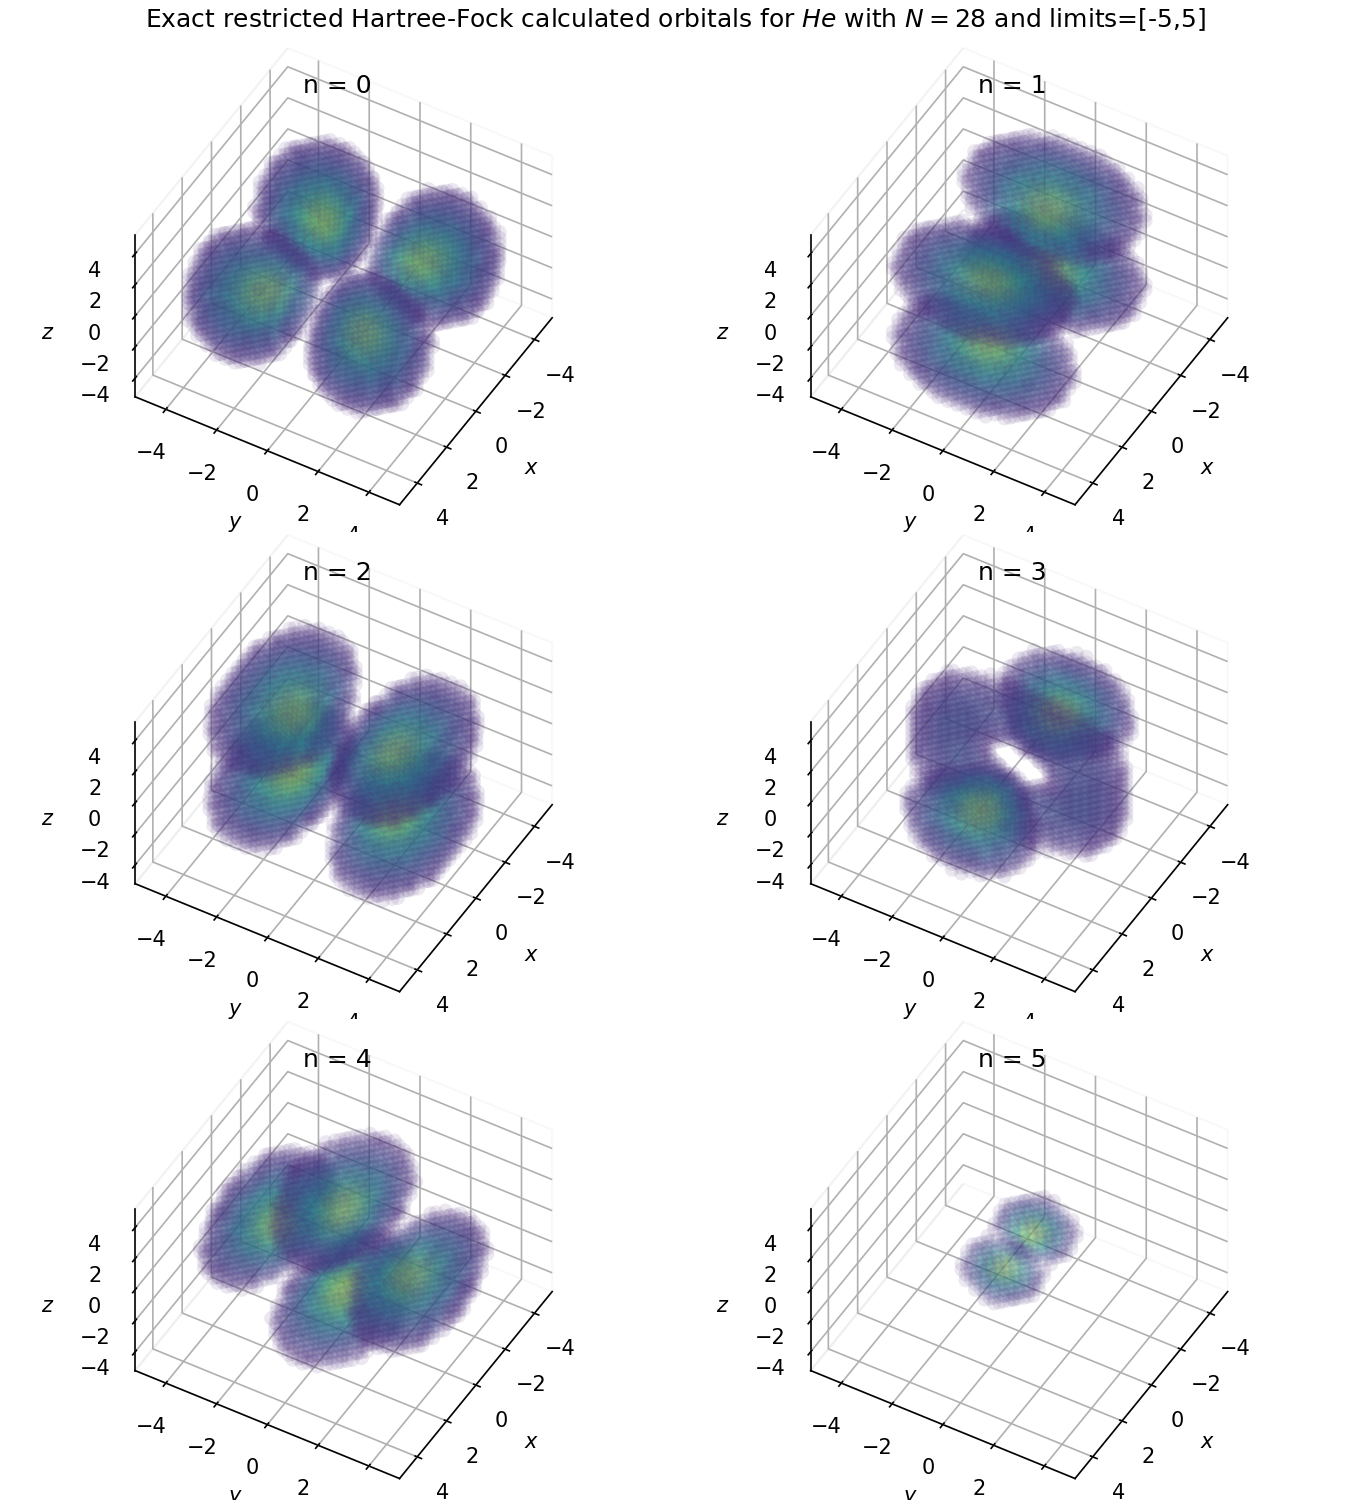
\includegraphics[scale=0.75]{he_N28_l5.png}
  \end{center}
  \caption{Calculated orbitals for $He$ atom using limits of [-5,5]}
  \label{he-plot-l5}
\end{figure}

\begin{figure}[H]
  \begin{center}
    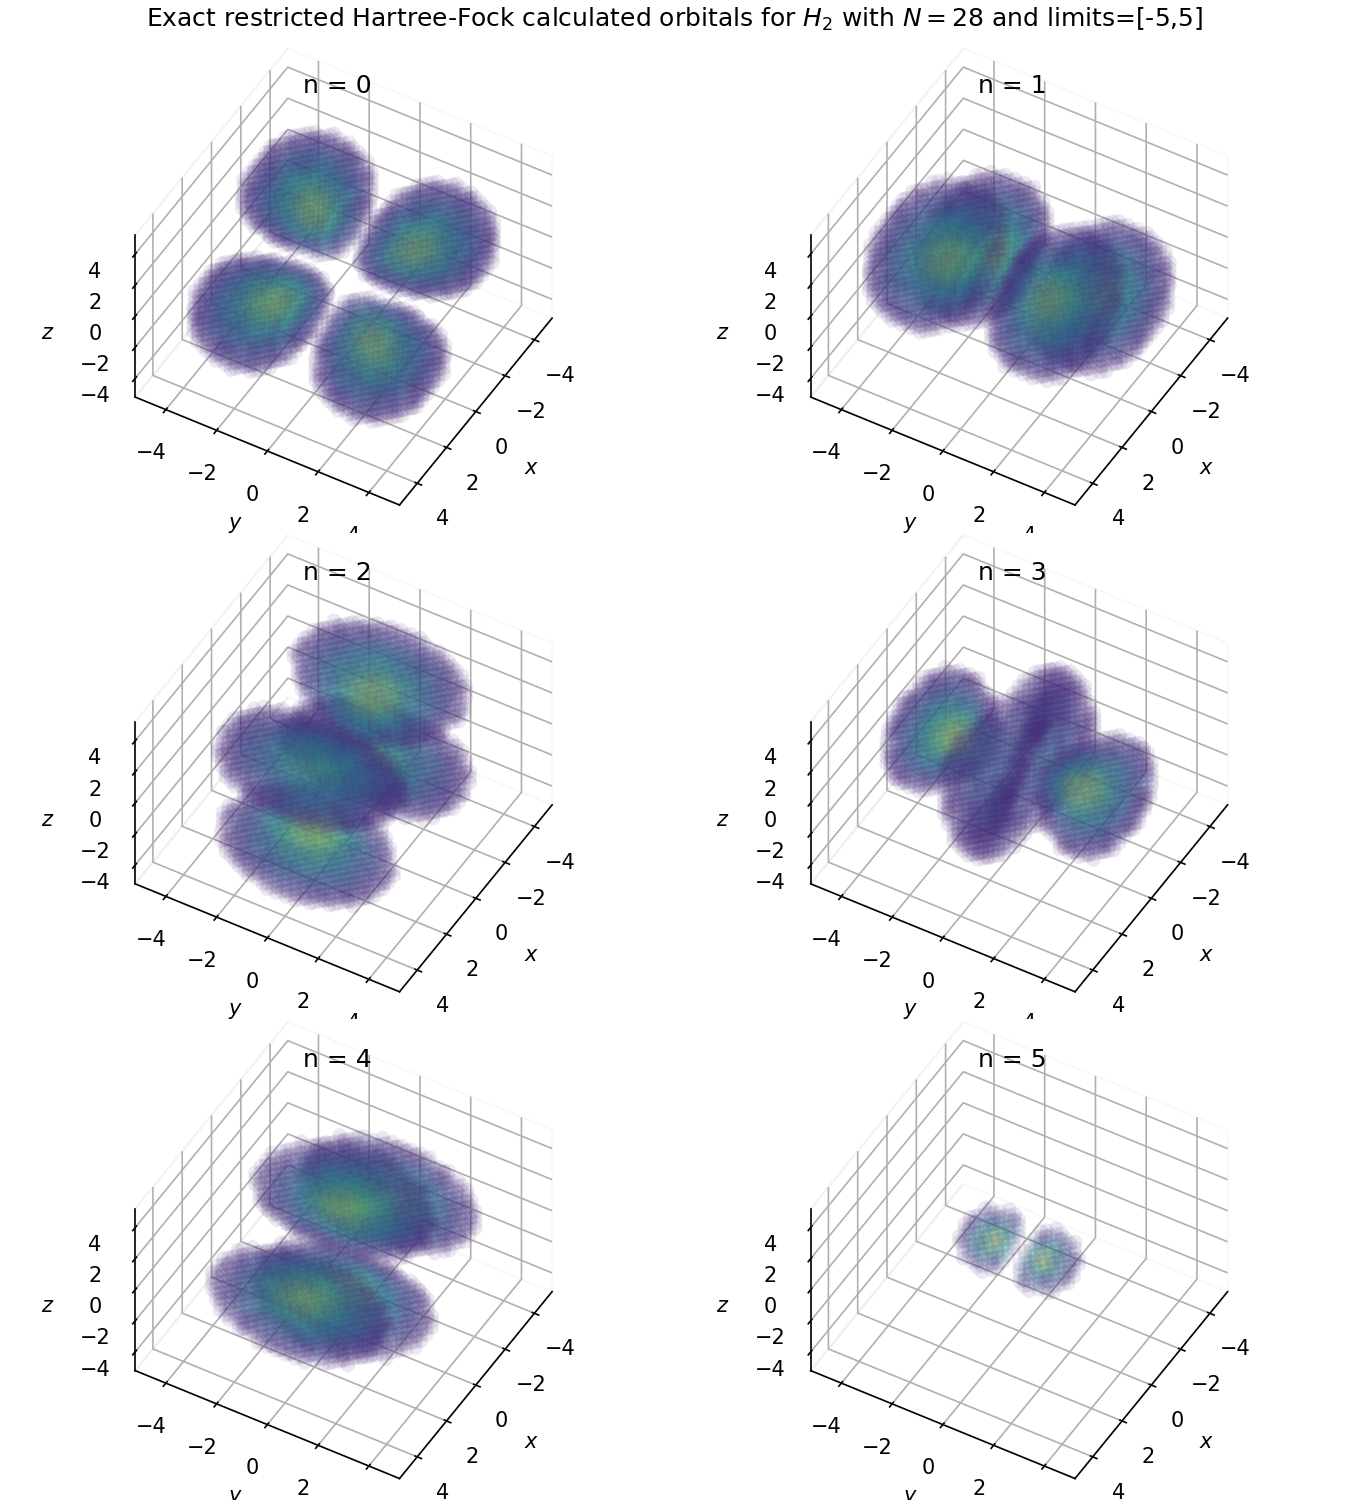
\includegraphics[scale=0.75]{h2_N28_l5.png}
  \end{center}
  \caption{Calculated orbitals for $H_2$ molecule using limits of [-5,5]}
  \label{h2-plot-l5}
\end{figure}

\begin{figure}[H]
  \begin{center}
    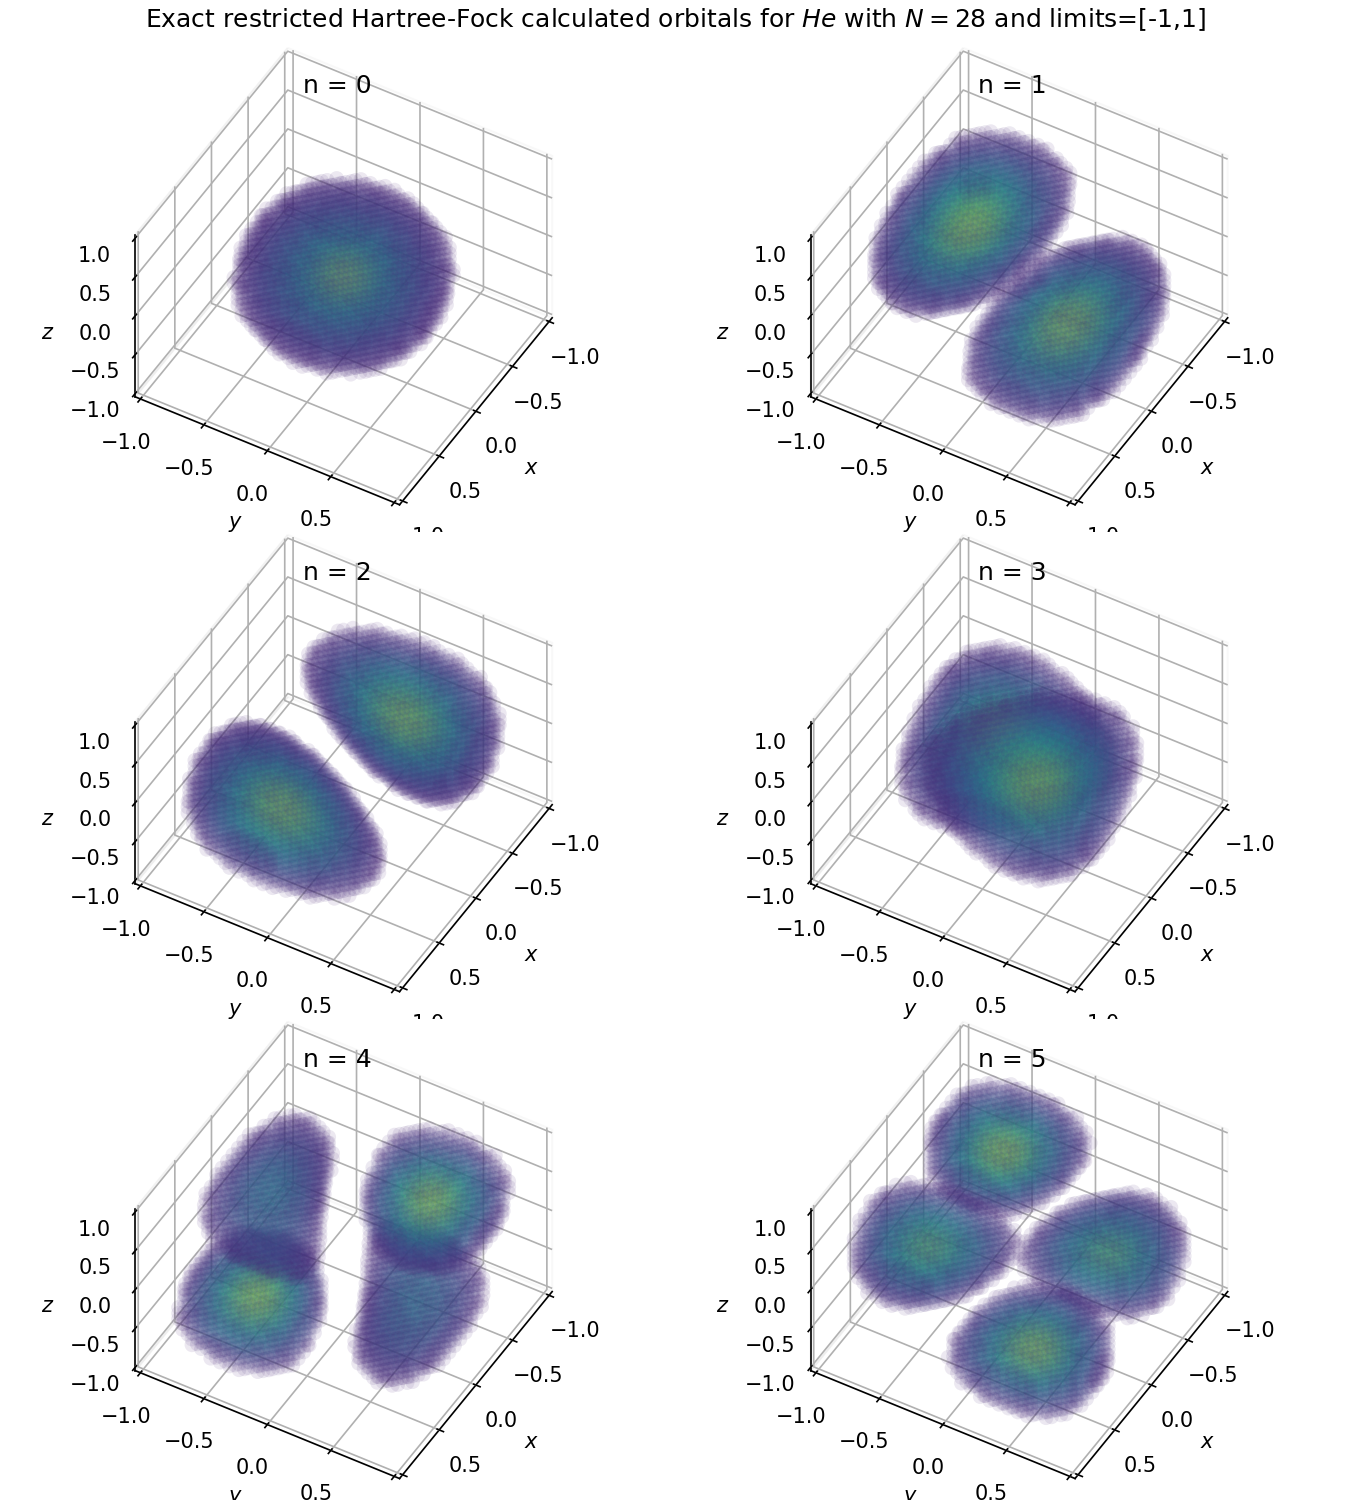
\includegraphics[scale=0.75]{he_N28_l1.png}
  \end{center}
  \caption{Calculated orbitals for $He$ atom using limits of [-1,1]}
  \label{he-plot-l1}
\end{figure}

\begin{figure}[H]
  \begin{center}
    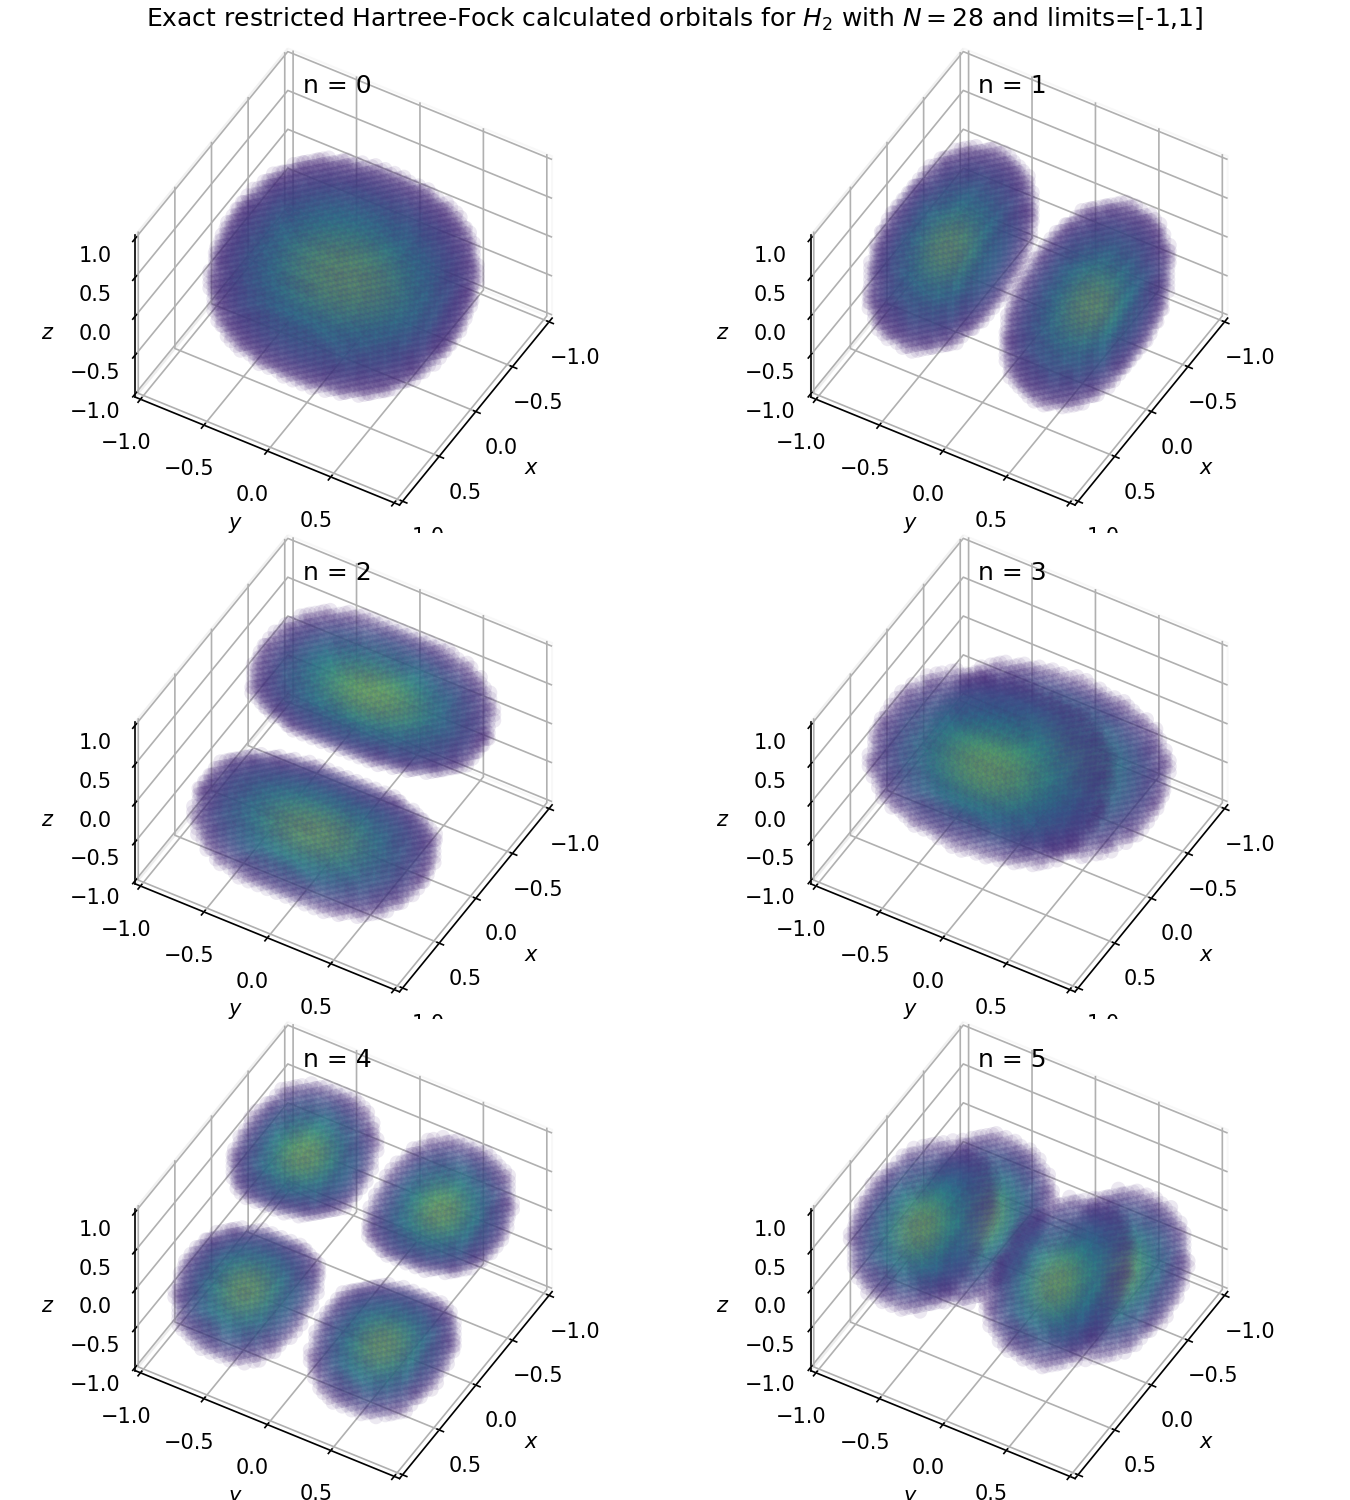
\includegraphics[scale=0.75]{h2_N28_l1.png}
  \end{center}
  \caption{Calculated orbitals for $H_2$ molecule using limits of [-1,1]}
  \label{h2-plot-l1}
\end{figure}

\begin{table}[H]
\begin{center}
\begin{tabular}{l|llllll}\hline
$n$    & $1$    & $2$     & $3$     & $4$      & $5$      & $6$      \\\hline
$E_n$  & $-0.049968$  & $-0.049878$  & $-0.041970$  & $0.011558$  & $-0.007816$  & $0.065703$ \\\hline
\end{tabular}
\end{center}
  \caption{The first six orbital energy levels obtained from applying HF to the Helium atom using limits of [-5,5]}
  \label{orbital-energies-he-l5}
\end{table}

\begin{table}[H]
\begin{center}
\begin{tabular}{l|llllll}\hline
$n$    & $1$    & $2$     & $3$     & $4$      & $5$      & $6$      \\\hline
$E_n$  & $-0.054140$  & $-0.044237$  & $-0.040912$  & $-0.019278$  & $0.000325$  & $0.036600$ \\\hline
\end{tabular}
\end{center}
  \caption{The first six orbital energy levels obtained from applying HF to the Hydrogen molecule using limits of [-5,5]}
  \label{orbital-energies-h2-l5}
\end{table}
 
\begin{table}[H]
\begin{center}
\begin{tabular}{l|llllll}\hline
$n$    & $1$    & $2$     & $3$     & $4$      & $5$      & $6$      \\\hline
$E_n$  & $0.007629$  & $3.942602$  & $3.942602$  & $3.942602$  & $7.489690$  & $7.489690$ \\\hline
\end{tabular}
\end{center}
  \caption{The first six orbital energy levels obtained from applying HF to the Helium atom using limits of [-1,1]}
  \label{orbital-energies-he-l1}
\end{table}

\begin{table}[H]
\begin{center}
\begin{tabular}{l|llllll}\hline
$n$    & $1$    & $2$     & $3$     & $4$      & $5$      & $6$      \\\hline
$E_n$  & $1.005352$  & $4.004340$  & $4.510553$  & $4.510553$  & $7.648020$  & $7.648020$ \\\hline
\end{tabular}
\end{center}
  \caption{The first six orbital energy levels obtained from applying HF to the Hydrogen molecule using limits of [-1,1]}
  \label{orbital-energies-h2-l1}
\end{table}

\newpage
\section{Discussion}

\begin{itemize}
    \item Obtaining these final results took several hours, with each run taking approximately 1h15m to converge on a result. With a partition size of $N=28$, the sparse matrices were $N \times N \times N = 21,952$ in row and column length, for a total of $481,890,304$ entries. The solver took very long to chug through these numbers. Many more hours were spent in the development phase trying to tweak and debug the program. This was an incredible challenge.
    \item Vastly different solutions were obtained when using smaller limits for the problem. This is likely tied to the problem being constrained into a virtual box of sorts where the electrons weren't free to orbit further. It is assumed that the more correct orbital results are those for when the limits are set to larger values.
    \item There were repeated eigenvalues (of approximately the same value) with very similar shapes. This is likely the solver finding identical or similar orbitals in different orientations. It was reassuring to see some familiar shapes in the orbitals that were previously spotted as illustrations in textbooks.
    \item As mentioned in the program implementation, the eigenvalue solver used in this program does not fully utilize the capabilities of the computer. Future improvements on this solver would likely involve a re-write in a compiled language like C and make use of matrix algebra packages that are optimized to run on multiple cores and make use of large memory pools. This would help decrease the iteration speed and increase the possible resolution of the simulator.
    \item The current implementation does not treat the solution space as an infinite space and is more similar to a closed box. Either the limits need to be made large enough for the system or the implementation needs to simulate a larger space. The numerical integration, for example, may be able to extend its range, to allow the "other" electron to smear further.
    \item The solutions are extremely sensitive to partition size and the limits of the problem. Since the solver only reports the first six lowest eigenvalues, it's likely that similar solutions get moved in and out of these six slots as the parameters change.
    \item Unfortunately, the theory behind the total energy and orbital energy was not understood in time to include in the report. This is why the eigenvalues representing the orbital energies are left as they are without any units. This is also why they are used as-is as the convergence criteria for the algorithm instead of the total energy of the system. The orbital energies do not sum the Hartree-Fock energy. Koopman's theorem states that in restricted Hartree-Fock, the energies associated with occupied orbitals approximate the ionization energy of that orbital, and the energies associated with unoccupied orbitals approximate the energy required to place an electron into that orbital. The total energy of the system must be calculated using the following equation which accounts for the double contribution of electrons in the double electron integrals (hence the $\frac{1}{2}$):
    \begin{align*}
      E_o &= \sum_i^N\bra{i}\hat{h}\ket{i} + \frac{1}{2}\sum_i^N\sum_j^N\bra{ij}\ket{ij}
    \end{align*}
    Since $N=2$ for both the Helium atom and the Hydrogen molecule, we should be able to use the same expanded form:
    \begin{align*}
      E_o &= \bra{1}\hat{h}\ket{1} + \bra{2}\hat{h}\ket{2} + \frac{1}{2}\left[\bra{11}\ket{11} + \bra{12}\ket{12} + \bra{21}\ket{21} + \bra{22}\ket{22}\right]
    \end{align*}
\end{itemize}

\newpage
\section{Code Listings and Data}

\subsection{Python Code Listing}
\label{code-listing-python}
The following is the code written in Python to generate the solutions and plots used in this report.
\lstinputlisting[language=Python]{exact-hartree-fock-sim.py}

\newpage
\section{References}

These aren't citing anything, but they were useful in helping me figure out this assignment.

\begin{itemize}
  \item \url{https://www.12000.org/my_notes/mma_matlab_control/KERNEL/KEse83.htm} % laplacian matrix derivation
  \item \url{https://www.value-at-risk.net/numerical-integration-multiple-dimensions/} % numerical integration
  \item \url{https://chem.libretexts.org/Bookshelves/Physical_and_Theoretical_Chemistry_Textbook_Maps/Book%3A_Quantum_States_of_Atoms_and_Molecules_(Zielinksi_et_al)/09%3A_The_Electronic_States_of_the_Multielectron_Atoms/9.07%3A_The_Self-Consistent_Field_Approximation_(Hartree-Fock_Method)} % good overview of HF
  \item \url{http://vergil.chemistry.gatech.edu/notes/hf-intro/hf-intro.html} % another good overview of HF
  \item \url{https://chem.libretexts.org/Bookshelves/Physical_and_Theoretical_Chemistry_Textbook_Maps/Physical_Chemistry_(LibreTexts)/08%3A_Multielectron_Atoms/8.07%3A_Hartree-Fock_Calculations_Give_Good_Agreement_with_Experimental_Data} % energy extraction

  % Other not relevant
  % \item https://physics.stackexchange.com/questions/20703/why-does-iteratively-solving-the-hartree-fock-equations-result-in-convergence
  % \item https://scicomp.stackexchange.com/questions/1297/why-does-iteratively-solving-the-hartree-fock-equations-result-in-convergence
  % \item https://nznano.blogspot.com/2018/03/simple-quantum-chemistry-hartree-fock.html % basis
  % \item https://github.com/CrawfordGroup/ProgrammingProjects
  % \item https://github.com/aromanro/HartreeFock
  % \item https://github.com/ipudu/SCFpy % solves using a basis set, can't use
  % \item https://medium.com/analytics-vidhya/practical-introduction-to-hartree-fock-448fc64c107b % solves using a basis set, can't use
  % \item https://adambaskerville.github.io/posts/HartreeFockGuide/ % relies on Roothaan basis functions, can't use
\end{itemize}

\end{document}

